\documentclass[conference]{IEEEtran}
\IEEEoverridecommandlockouts
\usepackage[style=ieee]{biblatex}
\usepackage{amsmath,amssymb,amsfonts}
\usepackage{pgfplots}
\usepackage{algorithmic}
\usepackage{graphicx}
\usepackage{textcomp}
\usepackage{xcolor}
\usepackage{pgfplots}
\pgfplotsset{compat=1.15}
\usepackage{mathrsfs}
\usetikzlibrary{arrows}
\usepackage{enumitem}

\addbibresource{ROB_Projekt.bib}

\begin{document}

\title{Haptisches Feedback eines Roboters durch virtuelle 3D-Modelle}

\author{
    \IEEEauthorblockN{Carl Gathmann}
    \IEEEauthorblockA{\textit{Universität zu Lübeck}\\
        Lübeck, Germany \\
        carl.gathmann@student.uni-luebeck.de}
    \and
    \IEEEauthorblockN{Marten Buchmann}
    \IEEEauthorblockA{\textit{Universität zu Lübeck}\\
        Lübeck, Germany \\
        marten.buchmann@student.uni-luebeck.de}
}
\maketitle

\begin{abstract}
In dieser Studie wird ein Ansatz zur Erzeugung von haptischem Feedback im Bereich der 
Mensch-Roboter-Interaktion vorgestellt. 
Mittels Software wird eine sensorische Wahrnehmung simuliert, die durch frei gestaltbare, 
virtuelle 3D-Modelle gesteuert wird. Der Anwender erfährt eine Art abweisende Kraft, die durch die räumlichen 
Grenzen des virtuellen Modells definiert ist. Dadurch ist es möglich eine physische Interaktion mit dem immateriellen Modell 
nachzuahmen. Die vorgestellte Technologie findet viele Anwendungsbereiche. Von medizinischen 
Simulationen und Exploration in gefährlichen Zonen bis hin zur Erhöhung der Spielerfahrung in virtuellen Umgebungen.  

\end{abstract}

\begin{IEEEkeywords}
    Robotik, Haptisches Feedback 
\end{IEEEkeywords}

\section{Einleitung}
Die Mensch-Roboter-Interaktion hat in den letzten Jahren zunehmend an Bedeutung gewonnen und sich als ein 
dynamisches Forschungs- und Anwendungsfeld etabliert. Im Zentrum dieser Interaktion steht die Verbesserung 
der Benutzererfahrung durch die Erweiterung der sinnlichen Wahrnehmung des Menschen.

In dieser Studie wird eine Methode präsentiert, der es dem Benutzer ermöglicht, virtuelle 3D-Modelle zu 
"ertasten", indem über ein Roboterinterface mit diesen interagiert. Dies wird durch die Erzeugung einer 
abweisenden Kraft erreicht, die auf den Oberflächen der virtuellen Modelle basiert. Dieses haptische 
Feedback simuliert das physische Berühren eines realen Objekts, obwohl kein tatsächlicher physischer 
Kontakt mit dem Modell besteht. 

Dieser Ansatz bietet zahlreiche Anwendungsmöglichkeiten, darunter die Simulation von Operationen 
für Ausbildungszwecke, die Erkundung von Objekten in gefährlichen oder unzugänglichen Umgebungen und 
die Erhöhung der Immersion in virtuellen Spielen. Darüber hinaus kann die Kombination unserer Technologie 
mit Virtual-Reality-Brillen zu einem verbesserten Gefühl von Präsenz und Realismus in virtuellen Umgebungen führen. 
Die in dieser Arbeit vorgestellten Prinzipien und Implementierungen können als Grundlage für weiterführende 
Forschungen und Entwicklungen auf diesem Gebiet dienen.

Das vorliegende Paper beleuchtet die zugrundeliegenden Prinzipien, technische Details und potenzielle 
Anwendungen dieses Ansatzes.


\section{Methoden}
Die Erzeugung des haptischen Feedbacks beruht auf der Berechnung einer abweisenden Kraft, die so 
konzipiert ist, dass dem Benutzer ein realistisches Gefühl für die Form des virtuellen 3D-Modells 
vermittelt wird. Die Modelle können als Datei im STL-Standart übergeben werden. Der STL-Standart 
speichert 3D-Modelle als Dreiecksmesh, das aus Eckpunkten und den Normalen der Dreiecke besteht. 
Es ist keine besondere CAD Software nötig um 3D-Modelle im STL Format zu erstellen. Außerdem ist das 
Format weit verbeitet und wird in der Industire zur Speicherung und Übertragung von 3D-Modellen eingesetzt. 
Das sorgt für hohe Flexibilität und einfache Handhabung \autocite{WasIstSTLDatei2017}.

Für die physische Implementierung der Mensch-Roboter-Interaktion wurde der Panda-Roboter von 
Franka Emika ausgewählt. Der Panda verfügt über 7 DOF und Kraftsensoren in allen sieben Achsen. So bietet der 
Manipulator eine hohe 
Präzision und Flexibilität, aber auch einen gewissen Sicherheitstandart \cite{pandaDatasheet}. Eine benutzerfreundliche, 
3D-gedruckte Schnittstelle (siehe \ref{fig:MRinterface}) 
ist am Endeffektor des Roboters installiert, um die Führung durch menschliche Benutzer zu erleichtern.  

\begin{figure}
    \centering
    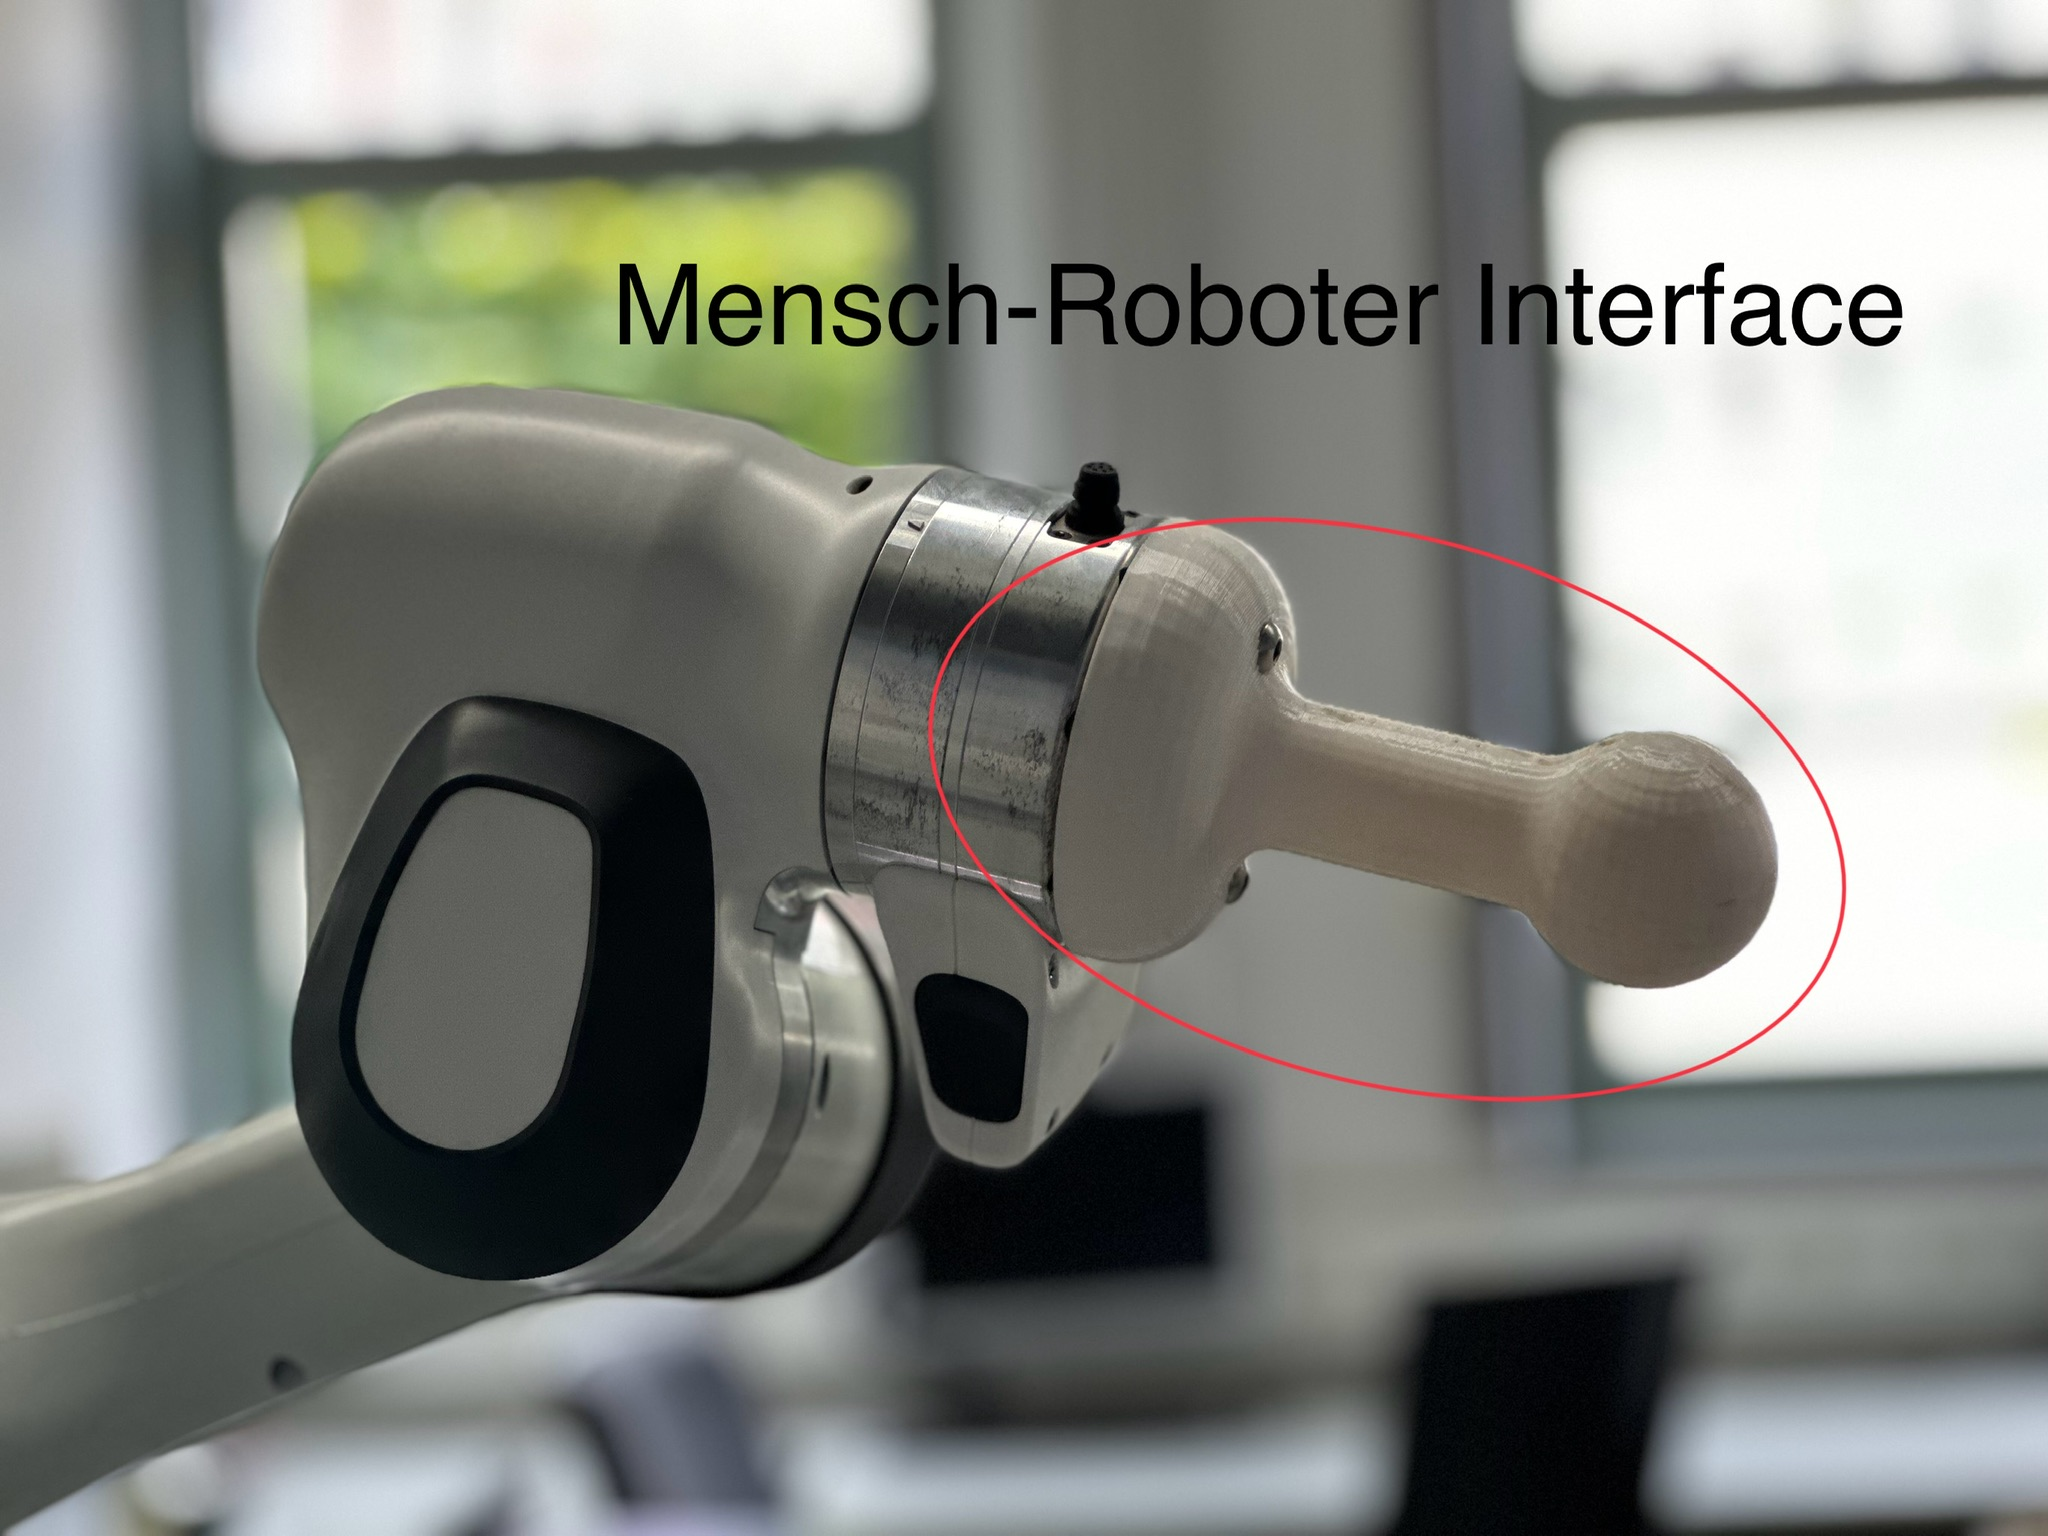
\includegraphics[width=0.45\textwidth]{pics/interface.jpeg}
    \caption{Mensch-Roboter-Schnittstelle}
    \label{fig:MRinterface}
\end{figure}

Bei der entwickeleten Software für dieses System ist die Leistungsfähigkeit äußerst kritisch, 
um eine nahtlose Benutzererfahrung zu gewährleisten. Es ist entscheidend, dass die Anwendung in 
Echtzeit ausgeführt werden kann, wobei eine maximale 
Zeitverzögerung von weniger als 1 Millisekunde akzeptiert wird. Die Programmiersprache 
C++ eignet sich aufgrund ihrer hohen Performance, um diesem Anspruch gerecht zu werden. 
Die Hardware-Konfiguration besteht aus !!!HARDWARE!!!.
Ein STL-Parser extrahiert die Eckpunkte der einzelen Dreiecke aus der STL-Datei und speichert diese in Matrizen. 
Damit eine einfache sowie effiziente Handhabung der 3D-Daten innerhalb des Programms möglich bleibt, werden 
Datentypen und Funktionen aus der "Eigen" Bibliothek verwendet. 

Im folgenden Teil werden verschieden Ansätze zur Erstellung eines stetigen und kontinuierlichen Vektorfeldes aus einem 
Dreiecksmesh vorgestellt. 

Für die Verwendung der Ansätze \ref*{edge} und \ref*{bary} muss als Vorbereitung zuerst ein zweidimensionales 
Problem aus dem dreidimensionalen Problem gemacht werden. Erreicht wird dies durch die Erstellung eines neuen 
Koordinatensystems für jedes Dreieck, welches sich ergibt durch:
\begin{enumerate}
    \item Eine Kante des Dreiecks als x-Achse
    \item Das Kreuzprodukt der entstandenen Achse mit einem weiteren Vektor als z-Achse
    \item Das Kreuzprodukt der beiden entstandenen Achsen als y-Achse
\end{enumerate}
Die Koordinaten des Punktes werden dann in diesem Koordinatensystem angegeben. Auf diese Art 
repräsentieren die x- und y-Koordinaten die Position und die z-Koordinate die Entfernung des Punktes 
von der Ebene des Dreiecks. 

\subsection{Edge Function}\label{edge}
Die "Edge Function" oder "Kanten Funktion" ist eine häufig verwendete Funktion im Bereich der Computer-Grafik. Sie wird 
verwendet, um herauszufinden, wo sich ein Punkt relativ zu einer Kante befindet \autocite{pinedaParallelAlgorithmPolygon1988}. 
Definiert ist sie wie folgt:
\begin{equation}
    E_{i} = (x_{i+1} - x_{i})(y - y_{i}) - (y_{i+1} - y_{i})(x - x_{i})
\end{equation}
x, y sind die Koordinaten des Punktes, $x_{i}$, $y_{i}$ sind die Koordinaten des i-ten Eckpunktes 
des Dreiecks.
Im Fall eines Dreiecks mit den Eckpunkten $A$, $B$ und $C$ und einem Punkt $P$ ist der Punkt innerhalb 
des Dreiecks, wenn gilt:
\begin{equation}
    E_{AB} \geq 0 \land E_{BC} \geq 0 \land E_{CA} \geq 0
\end{equation}

Mit dem Wissen, ob ein Punkt innerhalb des Dreiecks liegt und der Höhe des Punktes, die über 
die z-Koordinate des transformierten Punktes gegeben ist, kann ein Kraftvektor berechnet werden. 
Dieser Kraftvektor zeigt in Richtung der Normalen des Dreiecks und ist proportional zur Höhe des Punktes. 
Die Kraft kann dann wie folgt berechnet werden:
\begin{equation}
    F = \frac{1}{z} \cdot n
\end{equation}
$z$ ist die z-Koordinate des Punktes, der innerhalb des Dreiecks liegt und $n$ ist die Normale dieses Dreiecks.

\subsection{Baryzentrische Koordinaten} \label{bary}
Eine weitere Methode ist die Verwendung von baryzentrischen Koordinaten. 
Diese Methode ist sehr ähnlich zur "Edge Function", da diese ebenfalls verwendet wird, um herauszufinden, 
wo sich ein Punkt relativ zu einem Dreieck befindet. Ein wichtiger Unterschied ist allerdings, dass 
außerdem die relative Position innerhalb des Dreiecks bestimmt werden kann. Berechnet werden die 
Koordinaten wie folgt:
\begin{equation*}
    \lambda_b = \pm\frac{|\Lambda(\triangle(Q,B,C))|}{|\Lambda(\triangle(A,B,C))|}
\end{equation*}
\begin{equation}
    \lambda_c = \pm\frac{|\Lambda(\triangle(A,Q,C))|}{|\Lambda(\triangle(A,B,C))|}
\end{equation}
\begin{equation*}
    \lambda_a = 1 - \lambda_1 - \lambda_2
\end{equation*}
A, B, C sind hierbei die Eckpunkte des Dreiecks und P die in das Koordinatensystem des Dreiecks 
transformierte Roboter Position. $\Lambda$ repräsentiert eine Funktion für den Flächeninhalt eines Dreiecks. 
$\lambda_1$, $\lambda_2$ und $\lambda_3$ sind die baryzentrischen Koordinaten des Punktes P, welche aussagen, 
wie weit der Punkt von den jeweiligen Eckpunkten entfernt ist. 
Wenn alle drei Koordinaten positiv sind, liegt der Punkt innerhalb des Dreiecks. Nun lässt sich ein 
Schwellwert festlegen, ab dem eine Interpolation zwischen den Kanten/Eckpunkten des Dreiecks stattfindet. 
Dazu ist es notwendig, für jede Kante zu wissen, welche Dreiecke sie enthält und welche Normalen diese 
Dreiecke haben. Das Gleiche gilt für die Eckpunkte. Anschließend kann die Kraft wie folgt 
berechnet werden:
\begin{equation*}
    F_{BC} = 
    \begin{cases} 
        \frac{\lambda_a}{S}\cdot N_{\triangle} + (1-\frac{\lambda_a}{S})\cdot N_{BC} &  0 < \lambda_a < \text{S} \\
        0 & \text{sonst.}
    \end{cases}
\end{equation*}
\begin{equation*}
    F_{AC} = 
    \begin{cases} 
        \frac{\lambda_b}{S}\cdot N_{\triangle} + (1-\frac{\lambda_a}{S})\cdot N_{AC} &  0 < \lambda_b < \text{S} \\
        0 & \text{sonst.}
    \end{cases}
\end{equation*}
\begin{equation*}
    F_{AB} = 
    \begin{cases} 
        \frac{\lambda_c}{S}\cdot N_{\triangle} + (1-\frac{\lambda_a}{S})\cdot N_{AB} &  0 < \lambda_c < \text{S} \\
        0 & \text{sonst.}
    \end{cases}
\end{equation*}
$N_{\triangle}$ ist dabei die Normale des betrachteten Dreiecks und $N_{XY}$ sind dabei die Normalen der 
Dreiecke, die die jeweilige Kante XY enthalten. $S$ ist ein Benutzerdefinierter Schwellwert, ab dem die 
Interpolation stattfindet.
Die resultierende Kraft $F_{XY}$ ist die Kraft, die auf den Benutzer wirkt, wenn er sich auf der Kante 
zwischen den Punkten X und Y bewegt.

Für die Eckpunkte gilt ein ähnlicher Ansatz. Entsprechend wird die Kraft wie folgt berechnet:
\begin{equation*}
    F_{A} = 
    \begin{cases} 
        (1-\frac{\lambda_a}{S})\cdot N_{\triangle} + \frac{\lambda_a}{S}\cdot N_{A} &  S < \lambda_a < 1 \\
        0 & \text{sonst.}
    \end{cases}
\end{equation*} 
\begin{equation*}
    F_{B} = 
    \begin{cases} 
        (1-\frac{\lambda_b}{S})\cdot N_{\triangle} + \frac{\lambda_b}{S}\cdot N_{B} &  S < \lambda_a < 1 \\
        0 & \text{sonst.}
    \end{cases}
\end{equation*} 
\begin{equation*}
    F_{C} = 
    \begin{cases} 
        (1-\frac{\lambda_c}{S})\cdot N_{\triangle} + \frac{\lambda_c}{S}\cdot N_{C} &  S < \lambda_a < 1 \\
        0 & \text{sonst.}
    \end{cases}
\end{equation*} 

\subsection{Point-Triangle-Distance-Funktion}\label{dist}
Die tatsächlich angewandte Methode zur des Kraftvektors basiert auf den Ergebnissen 
von \Citeauthor{eberlyDistancePointTriangle}. In der Arbeit wird eine Methode zur Berechnung der Punkt-Dreieck-Distanz präsentiert. Die Methode liefert dabei zwei wesentliche Werte zurück:

\begin{enumerate}
\item 'dist': Dieser Parameter repräsentiert den minimalen Abstand zwischen einem vorgegebenen Punkt $P$ und dem Dreieck. Der Wert entspricht der kürzesten euklidischen Distanz, die von $P$ bis zur nächsten Position auf dem Dreieck (seien es Kanten, Eckpunkte oder eine Flächenposition innerhalb der Dreiecksgrenzen) 
gemessen wird.
\item 'foot': Dieser Parameter repräsentiert den entsprechenden Punkt auf dem Dreieck, der $P$ am nächsten liegt. Es handelt sich hierbei um den Punkt auf dem Dreieck, der den minimalen Abstand 'dist' zu $P$ aufweist.
\end{enumerate}


\begin{figure}[h] 
    \centering
    \begin{tikzpicture}
        \begin{axis}[
            xmin=-2, xmax=4,
            ymin=-2, ymax=4,
            axis lines=center,
            axis on top=true,
            domain=0:1,
            ylabel=$t$,
            xlabel=$s$,
            xtick=false,
            ytick=false,
            ]
            \addplot [dashed, line width = 1pt] coordinates {(-1,3) (3,-1)};
            \addplot [dashed, line width = 1pt] coordinates {(-1,0) (3.5,0)};
            \addplot [dashed, line width = 1pt] coordinates {(0,-1) (0,3.5)};

            \node at (axis cs:0.6,0.6) {R0};
            \node at (axis cs:1.5,1.5) {R1};
            \node at (axis cs:-0.5,3.25) {R2};
            \node at (axis cs:-0.5,1) {R3};
            \node at (axis cs:-0.5,-0.5) {R4};
            \node at (axis cs:1,-0.5) {R5};
            \node at (axis cs:3.25,-0.5) {R6};
        \end{axis}
    \end{tikzpicture}
    \caption{Die Unterteilung des Dreiecks in Regionen.}
    \label{fig:regions}
\end{figure}


Die Anwendung dieser Methode ermöglicht somit eine präzise und effiziente Bestimmung der Punkt-Dreieck-Distanz im dreidimensionalen Raum.
Um dieses Ergebnis zu erreichen wird zunächst die Darstellungsform des Dreiecks verändert. Die Eckpunkte eines Dreiecks werden in eine Ebenengleichung $ T(s,t) = B + sE_0 + tE_1 $ übertragen, wobei $(s, t) \in D = \{(s,t): s \geq 0, t \geq 0, s + t \leq 1 \}$ gelten muss. Die Entfernung $Q(s,t)$ zwischen einem Punkt $P$ und dem Dreieck $T(s,t)$ lässt sich durch den quadrierten euklidischen Abstand als elliptischen Paraboloid darstellen: 
\begin{equation}
    Q(s,t) = |T(s,t) - P|^2 = as^2 + 2bst + ct^2 + 2ds + 2et + f
\end{equation}
mit $(s,t) \in D$. Die Koeffizienten $a, b, c, d, e, f$ lassen sich durch die Eckpunkte des Dreiecks und den Punkt $P$ berechnen \autocite*{eberlyDistancePointTriangle}. Somit kann die Punkt-Dreieck-Distanz durch die Minimierung von $Q(s,t)$ bestimmt werden. Durch die Annahme, dass $E_0$ und $E_1$ linear unabhängig sind kann $Q(s,t)$ nur ein globales Minimum besitzen. Das Minimum von $Q(s,t)$ kann durch das Nullsetzen des Gradienten  ermittelt werden. Daraus ergeben sich die Parameter $\tilde{t} = \frac{be-cd}{ac-b^2}$ sowie $\tilde{s} = \frac{bd-ae}{ac-b^2}$. Sind $(\tilde{s}, \tilde{t}) \in D$, so ist der Fußpunkt 'foot' des Punktes $P$ innerhalb des Dreiecks. Andernfalls muss der Fußpunkt auf den Kanten oder Eckpunkten des Dreiecks liegen. Um die korrekte Lage des Fußpunktes zu bestimmen wird das Dreieck wie in Bild \ref{fig:regions} in unterschiedliche Regionen unterteilt. Der genaue Fußpunkt wird mit Hilfe ellipsenförmiger Ebenenkurven bestimmt. Diese liegen in der $s, t$-Ebene, demnach ist $Q(s, t)$ dort konstant. Dies vereinfacht die Berechunungen ob der Fußpunkt auf einer Kante oder einem Eckpunkt liegt. Im wesentlichen muss für die Regionen R1, R3, R5 die Ebenenkurve gewählt werden, die die Kante des Dreiecks tangential schneidet. Das Minimum von $Q(s, t)$ ist dann für R1 $(s, t)$, für R3 $(0, t)$ und für R5 $(s, 0)$. Einen Sonderfall bilden die Regionen R2, R4 und R6. Hier muss ebenfalls die Richtung der Kante sowie die des Gradienten beachtet werden. Hier wird das Vorzeichen des Skalarprodukts der beiden Richtungen betrachtet um die Region des Fußpunktes zubestimmen. Es gilt für R2 $(1, -1) \cdot grad(Q(0, 1))$, für R4 $(1, 0) \cdot grad(Q(0, 0))$ und für R6 $(-1, 0) \cdot grad(Q(1, 0))$. 

\begin{figure}[h]
    \centering
    \begin{tikzpicture}
        \begin{axis}[
            xmin=-0.05, xmax=0.1,
            ymin=-0.2, ymax=1.2,
            axis lines=center,
            axis on top=true,
            domain=0:1,
            ylabel=$influence$,
            xlabel=$distance$,
            xticklabels=false,
            every axis x label/.style={
                at={(ticklabel* cs:1.05)},
                anchor=west,
            },
            ]
            \addplot [dashed, line width = 1.5pt] coordinates {(-0.04,1) (-0.02,1)};
            \addplot [line width=1pt] coordinates {(-0.02,1) (0.02,1)};
            \addplot [line width=1pt] coordinates {(0.02,1) (0.05,0)};
            \addplot [line width=1pt] coordinates {(0.05,0) (0.07,0)};
            \addplot [dashed, line width = 1.5pt] coordinates {(0.07,0) (0.09,0)};

            \addplot [dashed] coordinates {(0.02,1) (0.02,0)};

            \node[label={270:0.02},inner sep=1.5pt] at (axis cs:0.02,0) {};
            \node[label={0:{$A$}},circle,fill,inner sep=1.5pt] at (axis cs:0.02,1) {};
            \node[label={45:{$B$}},label={270:0.05},circle,fill,inner sep=1.5pt] at (axis cs:0.05,0) {};
            
        \end{axis}
    \end{tikzpicture}
    \caption{Die Funktion $influence(dist)$, die den Einfluss der Distanz auf den resultierenden Kraftvektor $F$ bestimmt.}
    \label{fig:influence}
\end{figure}

Um den resultierenden Kraftvektor zu ermitteln, wurde folgendes Verfahren implementiert: \\
\textbf{für jedes Dreieck der STL Datei:}
\begin{enumerate}
    \item Berechnung von $dist$ und $pp0$ mithilfe der Point-Triangle-Distance-Funktion.
    \item Berechnung des Vektors $v$ zwischen $pp0$ und der Roboterposition $p$.
    \item Wenn das Skalarprodukt von $v$ und der Normalen des Dreiecks positiv ist, wird die 
    resultierende Kraft $F$ wie folgt ergänzt:
    \begin{equation*}
        F \mathrel{\raisebox{0.19ex}{$\scriptstyle+$}}= v \cdot influence(dist)
    \end{equation*}
\end{enumerate}

Die Funktion $influence(dist)$ repräsentiert eine lineare Abschwächung innerhalb eines spezifischen Intervalls, das von 1 auf 0 abfällt (siehe Bild \ref{fig:influence}). So können die verschiedenen Einflüsse der Kraftvektoren auf den resultierenden Gesamtkraftvektor variiert werden. Ein breiteres Intervall führt dabei zu einer weicheren und abgerundeteren Haptik des simulierten Objekts. In unserer Implementierung haben wir ein Intervall von 5cm bis 2cm festgelegt. Vektoren, die von dem Punkt der minimalen Distanz zur Roboterposition ausgehen und eine Länge von weniger als 2 cm aufweisen, werden mit vollständiger Intensität in die Berechnung einbezogen. Vektoren mit einer Länge von 5 cm oder mehr werden aus der Berechnung ausgeschlossen. Für alle dazwischenliegenden Vektorlängen erfolgt eine lineare Interpolation.

\begin{figure}[h]
    \centering
    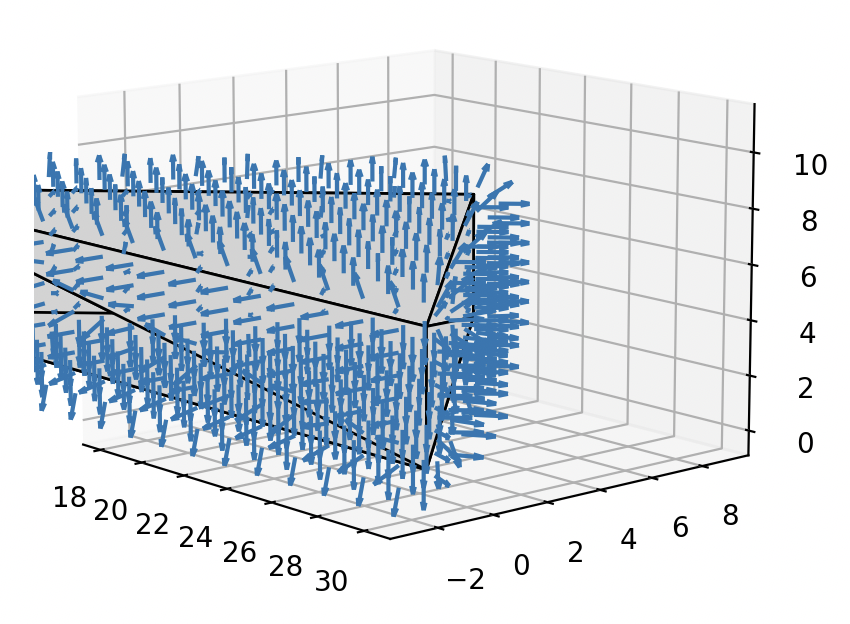
\includegraphics[width=0.5\textwidth]{pics/vectorfield.png}
    \caption{Vektorfeld, das resultierende Kräfte für verschiedene Punkte visualisiert.}
    \label{fig:vectorfield}
\end{figure}

Zur Visualisierung der Kräfte für verschiedene Punkte wurde ein Vektorfeld erstellt 
(siehe \ref{fig:vectorfield}). Man kann klar erkennen, dass keine Unstetigkeiten entlang der 
Kanten und Eckpunkten auftreten.


\section{Ergebnisse}

\subsection{Effekt}
Bei der Überprüfung unserer Implementierung konnten wir feststellen, dass der beabsichtigte Effekt der 
abstoßenden Kraft sowie das gewünschte Gefühl von Plastizität erfolgreich erreicht wurden. 
Die Kanten und Ecken der in der STL-Datei definierten Struktur waren deutlich wahrnehmbar. 
Ein kurzes Demonstrationsvideo, welches die Funktionsweise und das Resultat der angewandten 
Implementierung veranschaulicht, kann unter dem folgenden Link eingesehen werden:
\begin{minipage}{\textwidth}
    \nobreak\url{https://youtu.be/IhARjkxuTvw}.
\end{minipage}

\subsection{Performanz}
Hinsichtlich der Performanz wurden ebenfalls zufriedenstellende Resultate erzielt. Bei der Verarbeitung 
einer STL-Datei, welche 160 Dreiecke beinhaltet, betrug die durchschnittliche Berechnungszeit für den 
Kraftvektor eines Punktes lediglich 0.714 Millisekunden bei der oben beschriebenen Hardware. Im Kontext 
einer Echtzeitanwendung stellt dieser Wert eine akzeptable Berechnungslast dar. 

\section{Diskussion}
Bei den Ansätzen \ref*{edge} und \ref*{bary} ist es schwierig ein lückenloses Vektorfeld zu erstellen. 
Die Methode aus \ref*{edge} besticht mit Einfachheit und Geschwindigkeit. Allerdings bietet  diese keine Möglichkeit, 
zwischen den einzelnen Dreiecken zu interpolieren. Daher enstehen Unstetigkeiten an den Kanten der Dreiecke, 
was zu unintuitivem und sprunghaftem Verhalten führen kann, wenn der Benutzer sich entlang der Kante 
bewegt.

Der Vorteil von baryzentrischen Koordinaten gegenüber der "Edge Function" ist, dass die Unstetigkeit 
entlang der Kanten vermieden werden. Die Berechnung der baryzentrischen Koordinaten ist jedoch komplexer und 
langsamer als die Berechnung der "Edge Function". Außerdem ist zum Interpolieren der unterschieldichen Dreieckflächen die 
Bestimmung der Nachbarschaftsbeziehungen notwedig. Dadurch ist der Rechenaufwand deutlich höher, was zur Verletzung 
der kritischen Laufzeit führen kann.

Auch die Methode \ref*{dist} kann unter bestimmten Umständen die nötige Laufzeit nicht einhalten. 
Sollten die STL-Dateien jedoch eine bestimmte Größe überschreiten und es wird keine leistungsfähigere 
Hardware eingesetzt, könnte die Anforderung an die Echtzeitfähigkeit nicht mehr zuverlässig erfüllt werden. 
Eine potenzielle Lösung hierfür könnte die Anwendung von Level of Detail (LOD) Modellen sein. 
Diese Modelle, die bei größerer Entfernung des Roboters zum Objekt genutzt werden können, zeichnen 
sich durch eine reduzierte Anzahl an Dreiecken aus und können demzufolge effizienter verarbeitet werden. 
Auch die Nutzung von Octrees könnte die Performance weiter verbessern, da durch deren Einsatz die Anzahl 
der zu verarbeitenden Dreiecke verringert werden kann. Ein Octree ist eine spezielle Art von Baumstruktur, 
die im Kontext der 3D-Computergrafik verwendet wird und eine effiziente räumliche Aufteilung ermöglicht. 
Durch die Anwendung dieser Methoden könnte die Leistungsfähigkeit des Systems auch bei umfangreicheren 
STL-Dateien erhalten bleiben und die Echtzeitanforderungen sicherstellen.

\section{Fazit}

Zusammenfassend kann gesagt werden, dass die Methode \ref*{dist} die nötige Performanz aufweist um ein 
haptisches Feedback zu erzeugen. Durch das Verwenden des STL-Standarts können mit Beschränkungen in der Auflösung des 
3D-Modells beliebige Objekte zu stetigen und kontinuierlichen Vektorfeldern konvertiert werden. Somit ist eine eine einfache und 
flexible Handhabung gewährleistet. Die Methode zur Erzeugung haptischen Feedbacks eines Roboters durch virtuelle 3D-Modelle 
kann demnach in unterschiedlichen Anwendungsbereich einzug finden.  

\printbibliography

\end{document}